\documentclass[compress, 9pt]{beamer}

\usepackage[T1,T2A]{fontenc}
\usepackage[utf8]{inputenc}
\usepackage[english,russian]{babel}
\usepackage{hyperref}
\usepackage{microtype}
\usepackage{csquotes}
\usepackage{amsmath}
\usepackage{amsthm}
\usepackage{amssymb}
\usepackage{mathtext}
\usepackage{physics}
\usepackage{newfloat}
\usepackage{caption}
\usepackage{indentfirst}
\usepackage{hyperref}
\usepackage{mdframed}
\usepackage{graphicx}
\usepackage{subfig}
\usepackage{appendix}
\usepackage{ragged2e} %% for \justifying

%% add hyphenation and word wrap to beamer slides
%% \justifying should explicitely be specified for
%% 'enumerate', 'itemize', etc.
\apptocmd{\frame}{}{\justifying}{}

%% add braces around equation number
\makeatletter
\let\oldtheequation\theequation
\renewcommand\tagform@[1]{\maketag@@@{\ignorespaces#1\unskip\@@italiccorr}}
\renewcommand\theequation{(\oldtheequation)}
\makeatother

%% workaround for the \@ifundefined macro update in the 2018 LaTeX release
%% should be fixed in one of the next releases of caption.sty
\makeatletter
\let\@@magyar@captionfix\relax
\makeatother

\DeclareGraphicsExtensions{.pdf,.png,.jpg,.PNG}
\graphicspath{{./img/}}
\captionsetup[figure]{justification=centering}
\renewcommand{\thesubfigure}{\asbuk{subfigure}}
\DeclareCaptionLabelSeparator{dotseparator}{. }
\captionsetup{labelsep=dotseparator}

\usepackage[%
    style=numeric,
    citestyle=numeric,
    isbn=true,
    url=true,
    defernumbers=true,
    %sorting=nyt, % sort by name, year, title
    sorting=none, % order of appearance
    bibencoding=utf8,
    backend=biber,
    language=auto, % get main language from babel
    autolang=other, % get item language from bib entry
]{biblatex}

\setbeamertemplate{background canvas}[vertical shading][bottom=red!2,top=green!2]

\usetheme{Ilmenau}
\usecolortheme{spruce}
\usefonttheme[onlysmall]{serif}

\setbeamercolor{title in head/foot}{parent=palette primary}
\setbeamercolor{author in head/foot}{parent=palette primary}
\setbeamercolor{institute in head/foot}{parent=palette primary}

\setbeamercolor{title}{fg=black}
\setbeamercolor{frametitle}{fg=black}
\setbeamercolor*{enumerate item}{fg=black}

\setbeamercolor*{bibliography item}{fg=black}
\setbeamercolor*{bibliography entry title}{fg=black}
\setbeamercolor*{bibliography entry author}{fg=black}
\setbeamercolor*{bibliography entry location}{fg=black}
\setbeamercolor*{bibliography entry note}{fg=black}

\setbeamertemplate{enumerate item}[default]
\setbeamertemplate{bibliography entry title}{}
\setbeamertemplate{bibliography entry location}{}
\setbeamertemplate{bibliography entry note}{}
\setbeamertemplate{bibliography item}{\insertbiblabel}

\addtobeamertemplate{navigation symbols}{}{%
    \usebeamerfont{footline}%
    \usebeamercolor[fg]{title}%
    \hspace{1em}%
    \insertframenumber/\inserttotalframenumber
}

\hypersetup{
    colorlinks,
    citecolor=black,
    filecolor=black,
    linkcolor=black,
    urlcolor=black
}

\AtBeginSection[]{
  \begin{frame}
  \vfill
  \centering
  \begin{beamercolorbox}[sep=8pt,center,shadow=true,rounded=true]{title}
    \usebeamerfont{title}\insertsection\par%
  \end{beamercolorbox}
  \vfill
  \end{frame}
}


\title{Презентация к отчету\\ по педагогической практике}
\author{Василевский~А.В.}
\institute[ННГУ]{Нижегородский университет им. Н.И.~Лобачевского}
\date{2020}

\bibliography{bibliography}

\begin{document}

    \frame[plain]{\titlepage}

    \begin{refsection}
    \section[Занятие первое]{Занятие первое\\
        {\LARGE{\textbf{\enquote{Методы анализа алгоритмов.\\ Классы сложности $P$ и $NP$}}}}\\
        по дисциплине \enquote{Мультимедиа-технологии}}

    \begin{frame}\frametitle{Общая характеристика}

        \begin{itemize}\justifying
            \item \textbf{Тип занятия.} Лекция.

            \item \textbf{Цель занятия.} Организация познавательной деятельности студентов для усвоения ими новых теоретических знаний об алгоритмах, методах их анализа, математических классах сложности, совершенствования имеющихся базовых навыков анализа алгоритмов.

            \item \textbf{Педагогические принципы.} Наглядности, научности, систематичности и последовательности, связи теории с практикой, сотрудничества, сознательности, активности и самодеятельности.

            \item \textbf{Форма организации студентов.} Фронтальная.

            \item \textbf{Средства обучения.} Компьютер с установленным программным обеспечением для просмотра презентаций, компьютерная презентация, проектор, экран.
        \end{itemize}

    \end{frame}

    \begin{frame}\frametitle{Образовательные задачи}

        \begin{itemize}\justifying
            \item Закрепление базовых знаний об алгоритмах и задачах.
            \item Закрепление знаний о простейших классификациях алгоритмов.
            \item Закрепление знаний о базовых свойствах алгоритмов.
            \item Закрепление знаний о простейших методах анализа алгоритмической сложности.
            \item Ознакомление студентов с методами анализа алгоритмов на предмет их корректности.
            \item Ознакомление студентов с понятиями машины Тьюринга и RAM-машины.
            \item Объяснение студентам понятия математического класса сложности задачи. Введение в проблематику \enquote{$P = NP$}.
            \item Формирование умений анализа задач на предмет определения класса сложности.
        \end{itemize}

    \end{frame}

    \begin{frame}\frametitle{Воспитательные задачи}

        \begin{itemize}\justifying
            \item Воспитание коммуникативных навыков студентов посредством обсуждения поставленных преподавателем вопросов, общения с преподавателем.
            \item Мотивирование на дальнейшее развитие навыков формального анализа алгоритмов.
            \item Побуждение к познавательной и научной деятельности.
        \end{itemize}

    \end{frame}

    \begin{frame}\frametitle{Развивающие задачи}

        \begin{itemize}\justifying
            \item Развитие способности применять теоретические знания для практического анализа конкретных примеров.
            \item Развитие навыков работы и анализа получаемой посредством презентации информации.
            \item Развитие внимания через анализ студентами конкретных примеров с использованием изложенного материала.
        \end{itemize}

    \end{frame}

    \begin{frame}\frametitle{Методы обучения}

        \begin{itemize}\justifying
            \item \textbf{По источнику информации и восприятию.} Словесные. Наглядные. Практические.
            \item \textbf{По логике мышления.} Дедуктивные. Индуктивные.
            \item \textbf{По степени самостоятельности и активности познавательной деятельности студентов.} Репродуктивные. Проблемно-поисковые. Исследовательские.
        \end{itemize}

    \end{frame}

    \begin{frame}\frametitle{Ход занятия}\footnotesize

        \begin{tabular}{| p{.18\textwidth} | p{.41\textwidth} | p{.33\textwidth} |}\hline
            {\textbf{Этап занятия}} &
            {\textbf{Деятельность преподавателя}} &
            {\textbf{Деятельность студентов}} \\ \hline

            \multicolumn{3}{|c|}{Организационный момент} \\ \hline

            {} &
            {Представляется студентам. Формулирует тему лекции, ставит задачи, намеченные на предстоящее занятие} &
            {Знакомятся с преподавателем. Вспоминают пройденный материал, лежащий в основе занятия} \\ \hline

            \multicolumn{3}{|c|}{Объяснение нового материала} \\ \hline

            {Базовые сведения об алгоритмах} &
            {Вводит понятия алгоритма, задачи, объясняет основные свойства алгоритмов и их основные классификации, направления и цели анализа алгоритмов} &
            {Вспоминают известные сведения об алгоритмах и их классификациях, усваивают новые системные знания} \\ \hline

            {Методы анализа корректности алгоритмов} &
            {В обзорном ключе объясняет возможные методы анализа корректности алгоритмов. Предлагает студентам самостоятельно ознакомиться с некоторыми наиболее важными системами формальной верификации и статического анализа алгоритмов (с указанием источников информации).} &
            {Заинтересовываются возможностью формальной верификации алгоритмов и статическим анализом программного кода} \\ \hline
        \end{tabular}

    \end{frame}

    \begin{frame}\frametitle{Ход занятия}\footnotesize

        \begin{tabular}{| p{.18\textwidth} | p{.41\textwidth} | p{.33\textwidth} |}\hline

            {Понятие и методы анализа алгоритмической сложности} &
            {Раскрывает понятие алгоритмической сложности, связанные с этим понятия машины Тьюринга и RAM-машины, способы анализа. Приводит простой пример расчета сложности для конкретного алгоритма (сортировки)} &
            {Вспоминают известные факты о сложности алгоритмов, необходимые математические сведения. Усваивают новый материал. Участвуют в разборе примера} \\ \hline

            {Классы сложности} &
            {Вводит понятие класса сложности задачи, приводит примеры задач и их класс сложности с разбором причин} &
            {Усваивают новый материал о классах сложности, соотносят материал данного пункта с материалом предыдущего} \\ \hline

            {Проблема \enquote{$P = NP$}} &
            {Ставит проблему гипотезы $P = NP$ и указывает на ее фундаментальную важность. Приводит следствия принятия данной гипотезы} &
            {Знакомятся с проблемой \enquote{$P = NP$}. Дополняют список возможных последствий равенства классов сложности $P$ и $NP$} \\ \hline

            \multicolumn{3}{|c|}{Контроль знаний} \\ \hline

            {Классы сложности} &
            {Предлагает студентам классифицировать набор задач, приведенный на слайдах презентации} &
            {Принимают совместное участие в решении поставленной задачи, участвуют в дискуссиях, обсуждают ошибки} \\ \hline
        \end{tabular}

    \end{frame}

    \begin{frame}\frametitle{Анализ занятия}

        \begin{itemize}\justifying
            \item Цели занятия достигнуты.
            \item Дидактические задачи решены.
            \item Выбранные методы, форма, средства обучения соответствуют типу и содержанию занятия.
            \item Фронтальная организация учащихся позволяет не только объяснить материал в отведенное время, но и организовать взаимодействие с преподавателем в рамках совместного решения небольших задач по теме занятия.
            \item В ходе занятия студенты выглядели серьезными, заинтересованными излагаемым материалом.
            \item Отведенное на занятие время и сложность некоторых вопросов занятия послужили ограничивающим фактором для более полного и глубокого раскрытия материала.
        \end{itemize}

    \end{frame}

    \begin{frame}\frametitle{Литература к занятию}
        \nocite{*}\printbibliography[heading=none, keyword={lesson1}]
    \end{frame}

    \end{refsection}

    \begin{refsection}
    \section[Занятие второе]{Занятие второе\\
        {\LARGE{\textbf{\enquote{Обратные задачи: условия корректности,\\ обратные задачи матфизики,\\ экстремальные задачи\\ для выпуклого функционала}}}}\\
        по дисциплине \enquote{Специальные главы математики}}

    \begin{frame}\frametitle{Общая характеристика}

        \begin{itemize}\justifying
            \item \textbf{Тип занятия.} Лекция.

            \item \textbf{Цель занятия.} Организация познавательной деятельности студентов для усвоения ими новых теоретических знаний об обратных задачах, выпуклых функционалах, множествах, функциях.

            \item \textbf{Педагогические принципы.} Наглядности, научности, систематичности и последовательности, сознательности.

            \item \textbf{Форма организации студентов.} Фронтальная.

            \item \textbf{Средства обучения.} Компьютер с установленным программным обеспечением для просмотра презентаций, компьютерная презентация, проектор, экран.
        \end{itemize}

    \end{frame}

    \begin{frame}\frametitle{Образовательные задачи}

        \begin{itemize}\justifying
            \item Закрепление базовых знаний об обратных задачах.
            \item Ознакомление студентов с элементами выпуклого анализа.
            \item Объяснение студентам классификации обратных задач с точки зрения теории систем.
            \item Ознакомление студентов с некоторыми обратными задачами математической физики.
            \item Формирование умений анализа задач на предмет корректности согласно условиям корректности.
        \end{itemize}

    \end{frame}

    \begin{frame}\frametitle{Воспитательные и развивающие задачи}

        \textbf{Воспитательные задачи:}

        \begin{itemize}\justifying
            \item Мотивирование на дальнейшее развитие навыков решения обратных задач.
            \item Побуждение к познавательной и научной деятельности.
        \end{itemize}

        \textbf{Развивающие задачи:}

        \begin{itemize}\justifying
            \item Развитие навыков работы и анализа получаемой посредством презентации информации.
            \item Развитие внимания.
        \end{itemize}

    \end{frame}

    \begin{frame}\frametitle{Методы обучения и ход занятия}

        \textbf{Методы обучения:}

        \begin{itemize}\justifying
            \item Словесные. Наглядные. Практические.
            \item Дедуктивные.
            \item Репродуктивные. Проблемно-поисковые.
        \end{itemize}

        \textbf{Ход занятия:}

        \begin{enumerate}\justifying
            \item Организационный момент
            \item Объяснение нового материала
            \begin{itemize}\justifying
                \item Выпуклые функции, функционалы, множества, операторы проекции на выпуклые множества
                \item Обратные задачи в теории систем и математической физике
                \item Корректность обратных задач
            \end{itemize}
        \end{enumerate}

    \end{frame}

    \begin{frame}\frametitle{Анализ занятия}

        \begin{itemize}\justifying
            \item Цели занятия достигнуты.
            \item Дидактические задачи решены.
            \item Выбранные методы, форма, средства обучения соответствуют типу и содержанию занятия.
            \item Фронтальная организация учащихся позволяет максимально раскрыть тему занятия и дать наиболее полную и общую информацию по теме за отведенное на занятие время.
            \item В ходе занятия студенты выглядели серьезными, интересующимися темой занятия и мотивированными на дальнейшее и более полное изучение и практическое применение полученных базовых знаний.
            \item При подготовке занятия преподаватель столкнулся с рядом трудностей, обусловленных, в основном, необходимостью уложить достаточно объемный и многогранный материал в отведенное на занятие время.
        \end{itemize}

    \end{frame}

    \begin{frame}\frametitle{Литература к занятию}
        \nocite{*}\printbibliography[heading=none, keyword={lesson2}]
    \end{frame}

    \end{refsection}

    \begin{frame}\frametitle{Фотография к отчету}
        \centering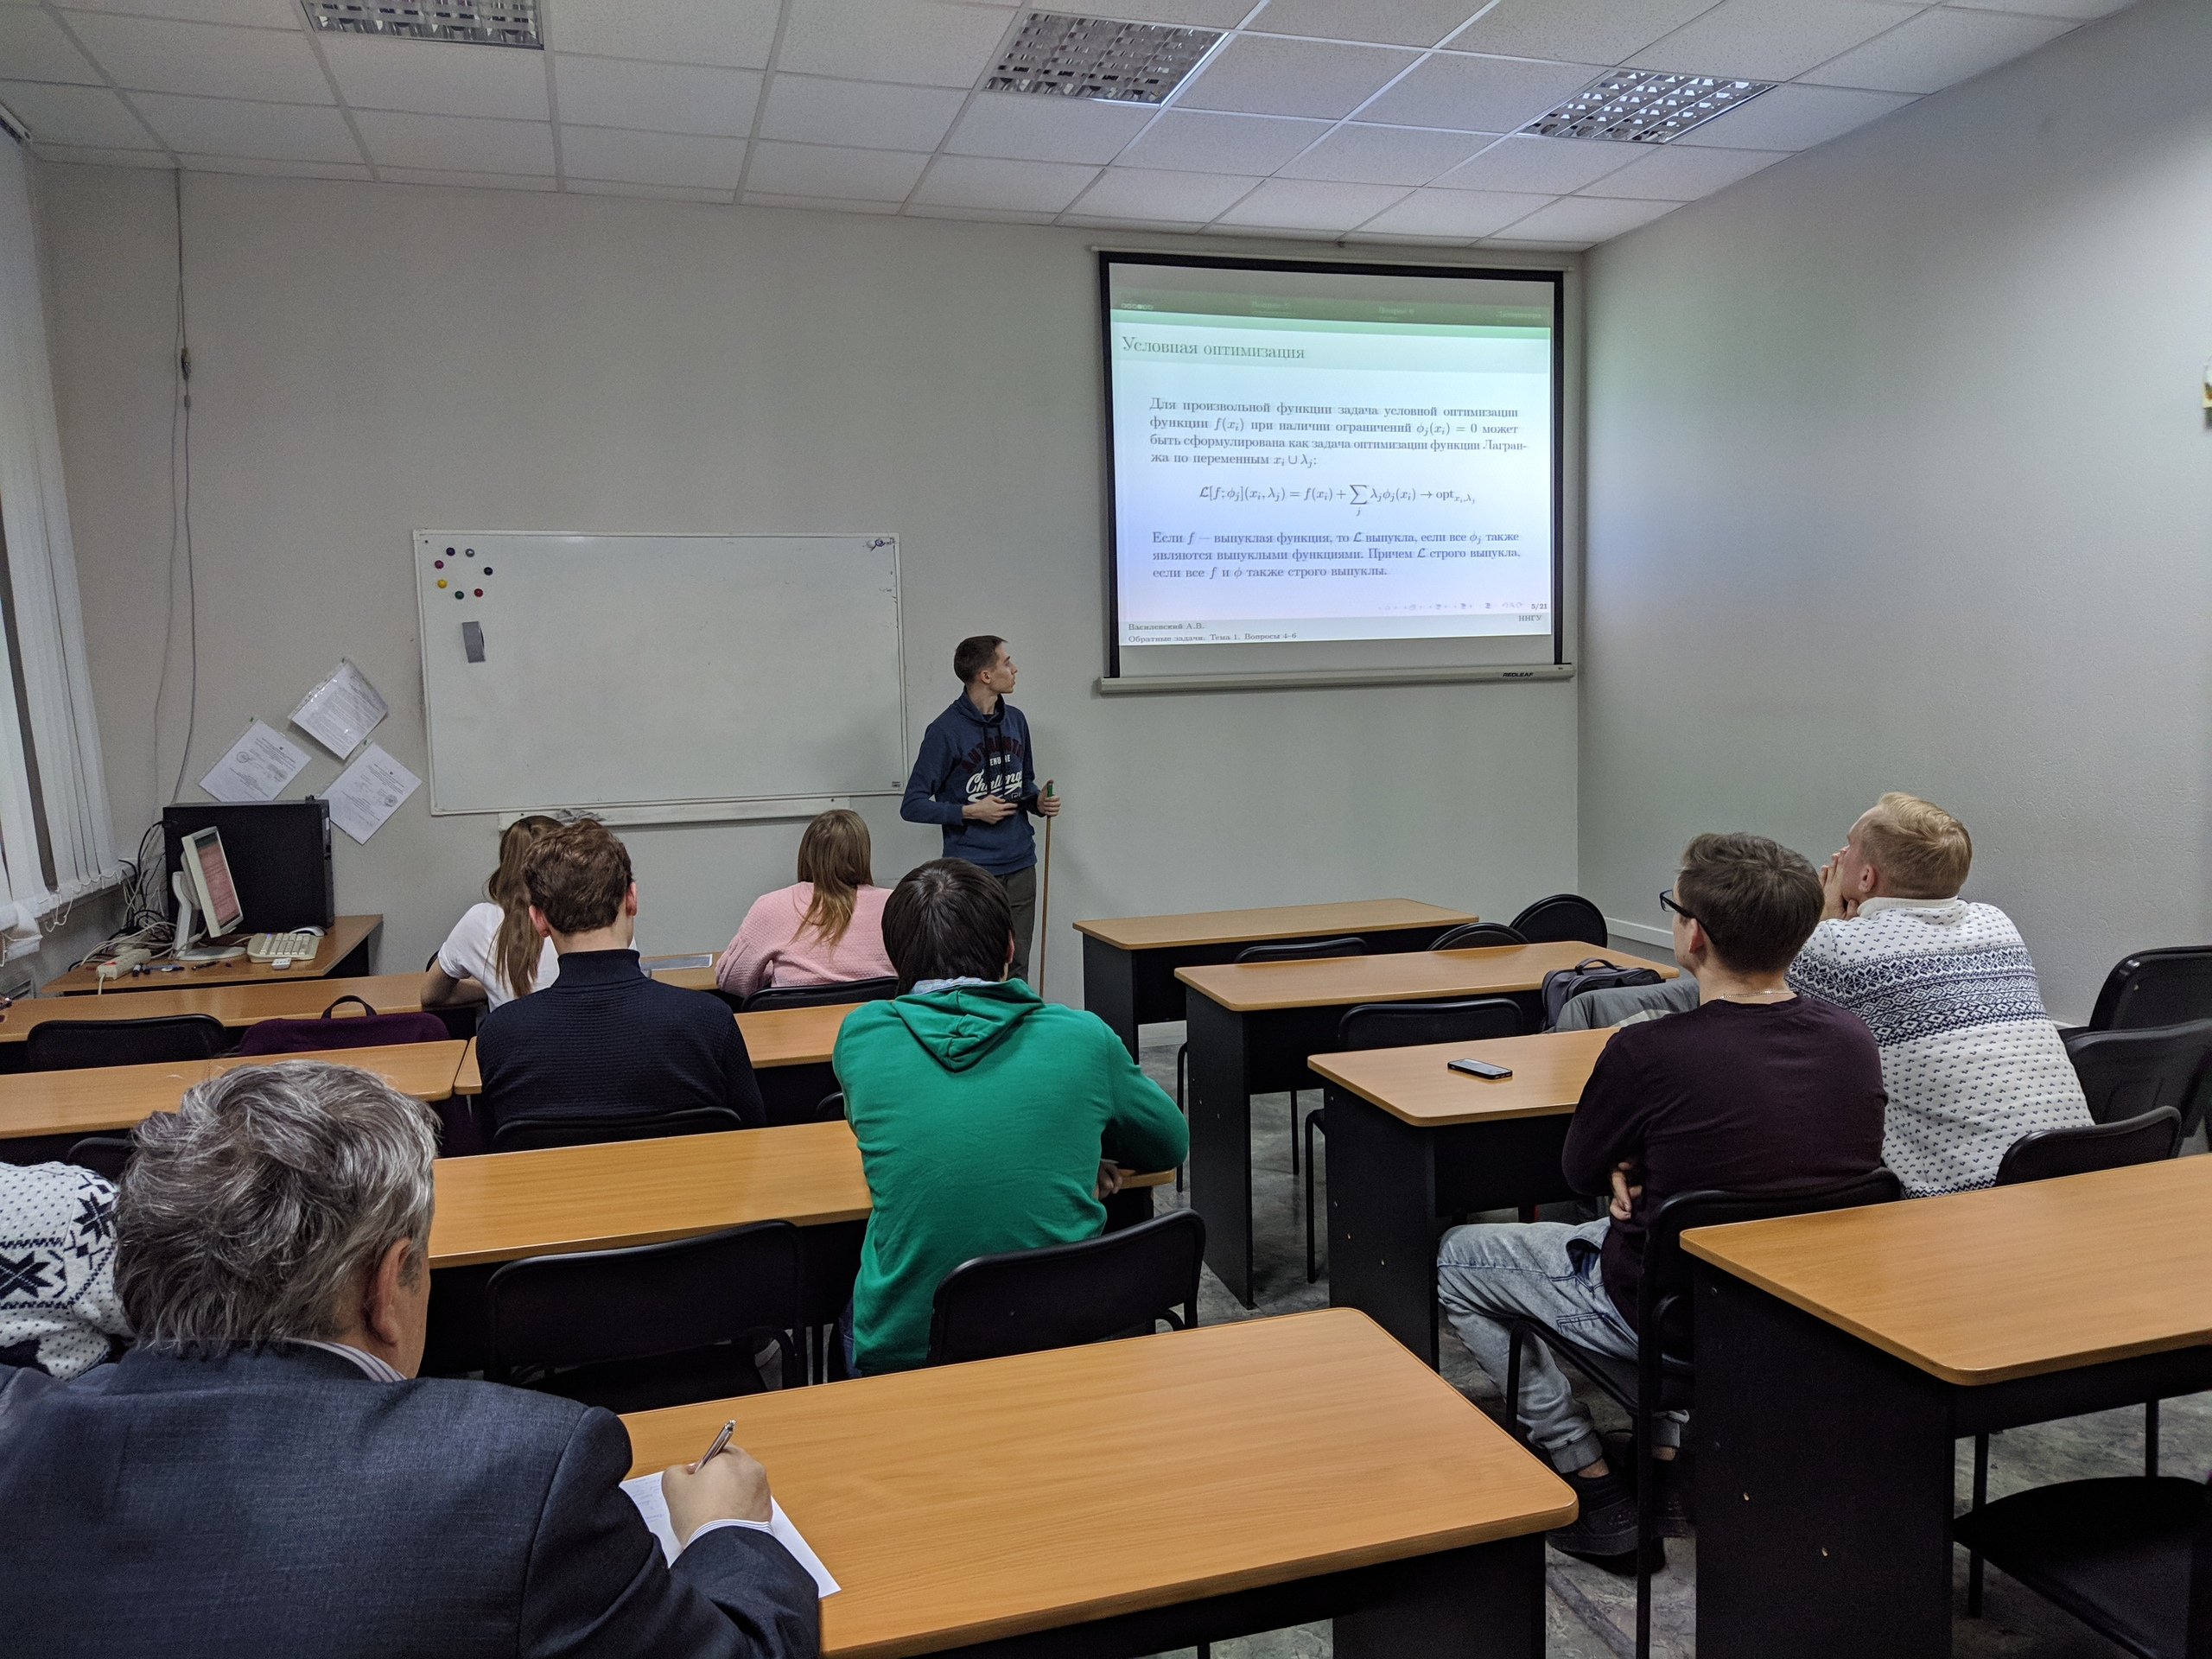
\includegraphics[width=\textwidth]{witness.jpg}
    \end{frame}

    \begin{frame}\frametitle{Литература}
        \nocite{*}\printbibliography[keyword={main}]
    \end{frame}

\end{document}
